\subsection{DNNの構成要素}
\subsubsection{全結合層}
全結合層は,入力に対して線型変換を施す層である.全結合層への入力を$\bm{\inputLower} \in \realSet^{\dimUpper_{\text{in}}}$とすると,出力$\bm{\outputLower} \in \realSet^{\dimUpper_{\text{out}}}$は,
\begin{equation}
    \bm{\outputLower} = \fcLayerValue{\bm{\inputLower}}{\bm{\weightAndBias}} = \lr{\bm{\inputLower}^{\top} \bm{\weightUpper}}^{\top} + \bm{\biasLower}
\end{equation}
で与えられる.ここで,$\dimUpper_{\text{in}}, \dimUpper_{\text{out}}$は入出力の次元,$\bm{\weightUpper} \in \realSet^{\dimUpper_{\text{in}} \times \dimUpper_{\text{out}}}$は重み,$\bm{\biasLower} \in \realSet^{\dimUpper_{\text{out}}}$はバイアスであり,$\bm{\weightAndBias}$は重みとバイアスをまとめて表す変数とする.また,入力が行列$\bm{\inputUpper} \in \realSet^{\timeUpper \times \dimUpper_{\text{in}}}$である時,出力$\bm{Y} \in \realSet^{\timeUpper \times \dimUpper_{\text{out}}}$は,
\begin{equation}
    \bm{\outputUpper} = \fcLayerValue{\bm{\inputUpper}}{\bm{\weightAndBias}} = \bm{\inputUpper} \bm{\weightUpper} + \bm{\biasLower} \bm{1}^{\top}
\end{equation}
で与えられる.ここで,$\timeUpper$は系列長,$\bm{1} \in \{1\}^{\timeUpper}$は全成分が1のベクトルである.全結合層はDNN内部での特徴量の次元の変換や,最終層において所望の出力に次元を合わせるのに用いられる.

\subsubsection{畳み込み層}
畳み込み層は,入力に対して畳み込み演算を行う層である.一次元畳み込み層について,入力を$\bm{\inputUpper} \in \realSet^{\dimUpper_{\text{in}} \times \timeUpper_{\text{in}}}$,出力を$\bm{\outputUpper} \in \realSet^{\dimUpper_{\text{out}} \times \timeUpper_{\text{out}}}$とし,それぞれ$\dimLower$次元目,$\timeLower$番目の成分を$\inputLower_{\dimLower_{\text{in}}, \timeLower}, \outputLower_{\dimLower_{\text{out}}, \timeLower}$で表す.$\dimUpper_{\text{in}}, \dimUpper_{\text{out}}$は入出力の次元,$\timeUpper_{\text{in}}, \timeUpper_{\text{out}}$は入出力の系列長である.このとき,$\outputLower_{\dimLower_{\text{out}}, \timeLower}$は,
\begin{align}
    \outputLower_{\dimLower_{\text{out}}, \timeLower} = b_{\dimLower_{\text{out}}} + \sum_{\dimLower_{\text{in}} = 1}^{\dimUpper_{\text{in}}} \sum_{\kernelSizeLower = 1}^{\kernelSizeUpper} \inputLower_{\dimLower_{\text{in}}, \timeLower - \lrFloor{\frac{\kernelSizeUpper}{2}} + \kernelSizeLower - 1} \weightLower_{\dimLower_{\text{in}}, \dimLower_{\text{out}}, \kernelSizeLower}
\end{align}
で与えられる.ここで,$\kernelSizeUpper$はカーネルサイズ,$\weightLower_{\dimLower_{\text{in}}, \dimLower_{\text{out}}, \kernelSizeLower}$は入力の$\dimLower_{\text{in}}$次元目から出力の$\dimLower_{\text{out}}$次元目に割り当てられたカーネルの$\kernelSizeLower$番目の成分,$b_{\dimLower_{\text{out}}}$は出力の$\dimLower_{\text{out}}$次元目に割り当てられたバイアスである.上式より,一次元畳み込み層の$\timeLower$番目の出力は,$\timeLower$番目を中心としたカーネルサイズの範囲分の入力から計算されることがわかる($\kernelSizeUpper$は奇数を想定した).これより,畳み込み層は入力の局所的な特徴を抽出するのに適した層だと考えられる.一次元畳み込みはテキストや音声など,データの形状が$\lr{\dimUpper \times \timeUpper}$となっている時に用いられる.

これに加えて,カーネルを二次元配列とすれば二次元畳み込み層,三次元配列とすれば三次元畳み込み層となる.二次元畳み込み層は画像など,データの形状が$\lr{\dimUpper \times \heightUpper \times \widthUpper}$となっている場合に用いられる.ここで,$\heightUpper$は高さ,$\widthUpper$を表す.三次元畳み込み層は動画など,データの形状が$\lr{\dimUpper \times \heightUpper \times \widthUpper \times \timeUpper}$となっている場合に用いられる.

畳み込み層における主要なパラメータは3つある.1つ目はカーネルサイズであり,これによって考慮できる入力特徴量の範囲が定まる.2つ目はストライドであり,これによってカーネルのシフト幅を設定できる.3つ目はダイレーションであり,これは畳み込み演算において計算対象となる入力特徴量の間隔を表す.ダイレーションを大きくすることで,カーネルサイズが同じでも考慮できる入力特徴量の範囲を広げることが可能である.また,出力系列長$\timeUpper_{\text{out}}$を入力系列長$\timeUpper_{\text{in}}$の整数倍に保つには,上記のパラメータに対して適切なパディング長を指定する必要がある.例えば,カーネルサイズを3,ストライドとダイレーションを1とした場合には,入力の両端に1ずつゼロパディングすれば良い.図~\ref{sec3:fig:conv_variations}に,ある次元における一次元畳み込み層の処理を示す.

\begin{figure}[tb]
    \centering
    \begin{subfigure}[b]{0.48\textwidth}
        \centering
        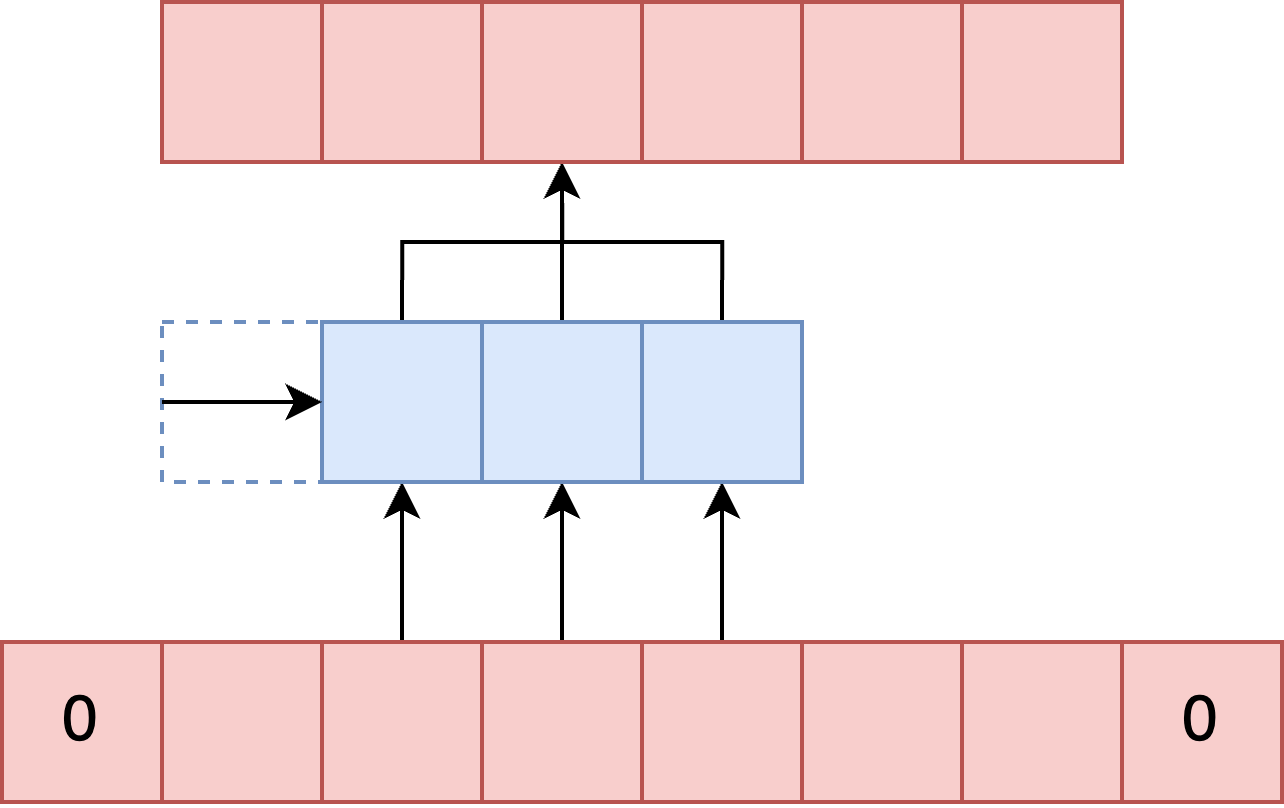
\includegraphics[height=4cm]{./figure/sec3/conv1.drawio.png}
        \caption{$\lr{\kernelSizeUpper, \strideUpper, \dilationUpper} = \lr{3, 1, 1}$}
        \label{sec3:fig:conv1}
    \end{subfigure}
    \begin{subfigure}[b]{0.48\textwidth}
        \centering
        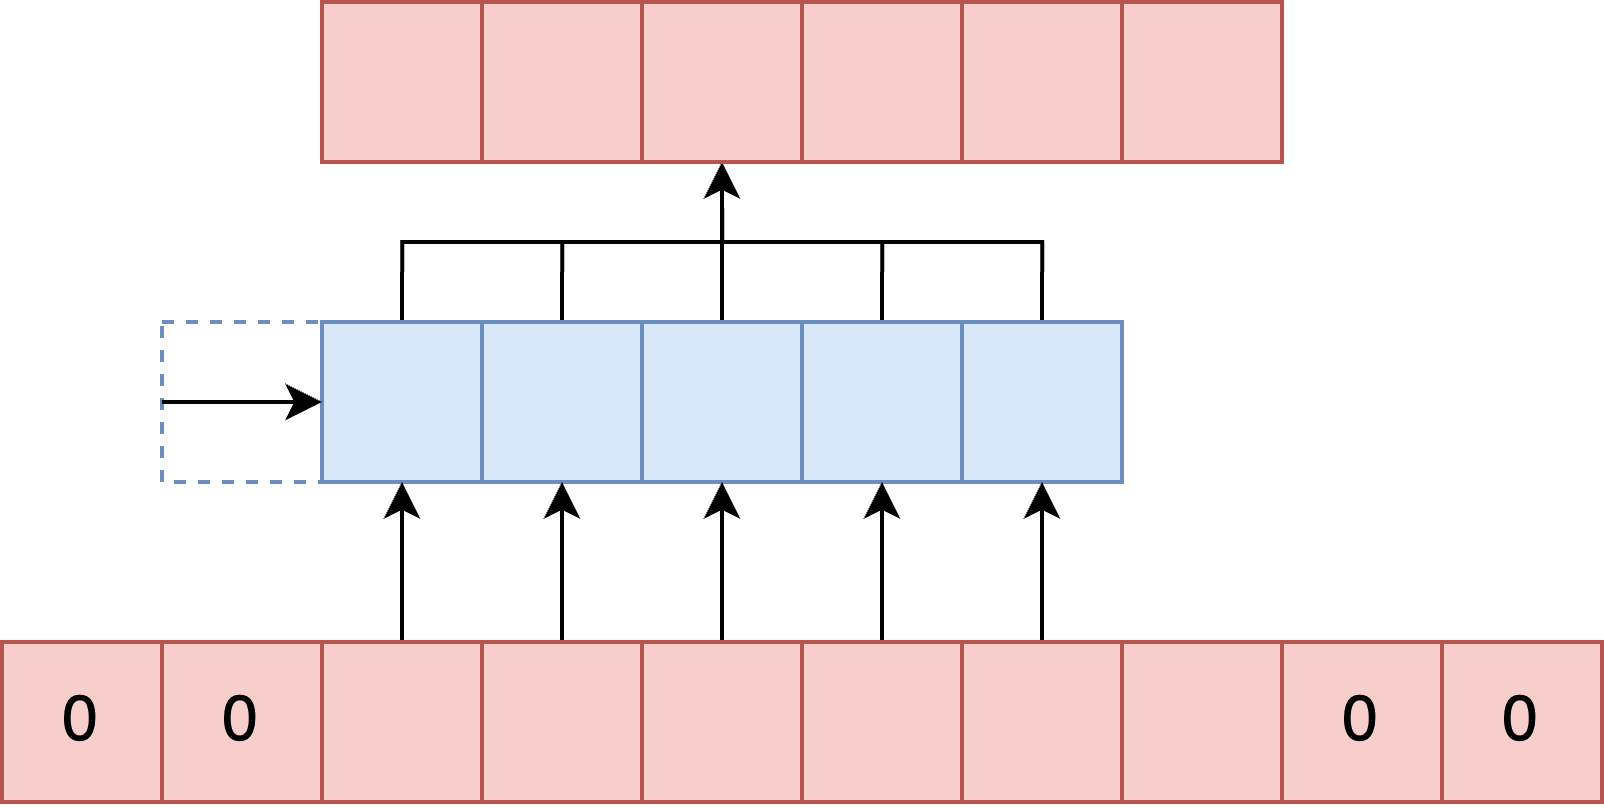
\includegraphics[height=4cm]{./figure/sec3/conv2.drawio.png}
        \caption{$\lr{\kernelSizeUpper, \strideUpper, \dilationUpper} = \lr{5, 1, 1}$}
        \label{sec3:fig:conv2}
    \end{subfigure}

    \vspace{0.5cm}

    \begin{subfigure}[b]{0.48\textwidth}
        \centering
        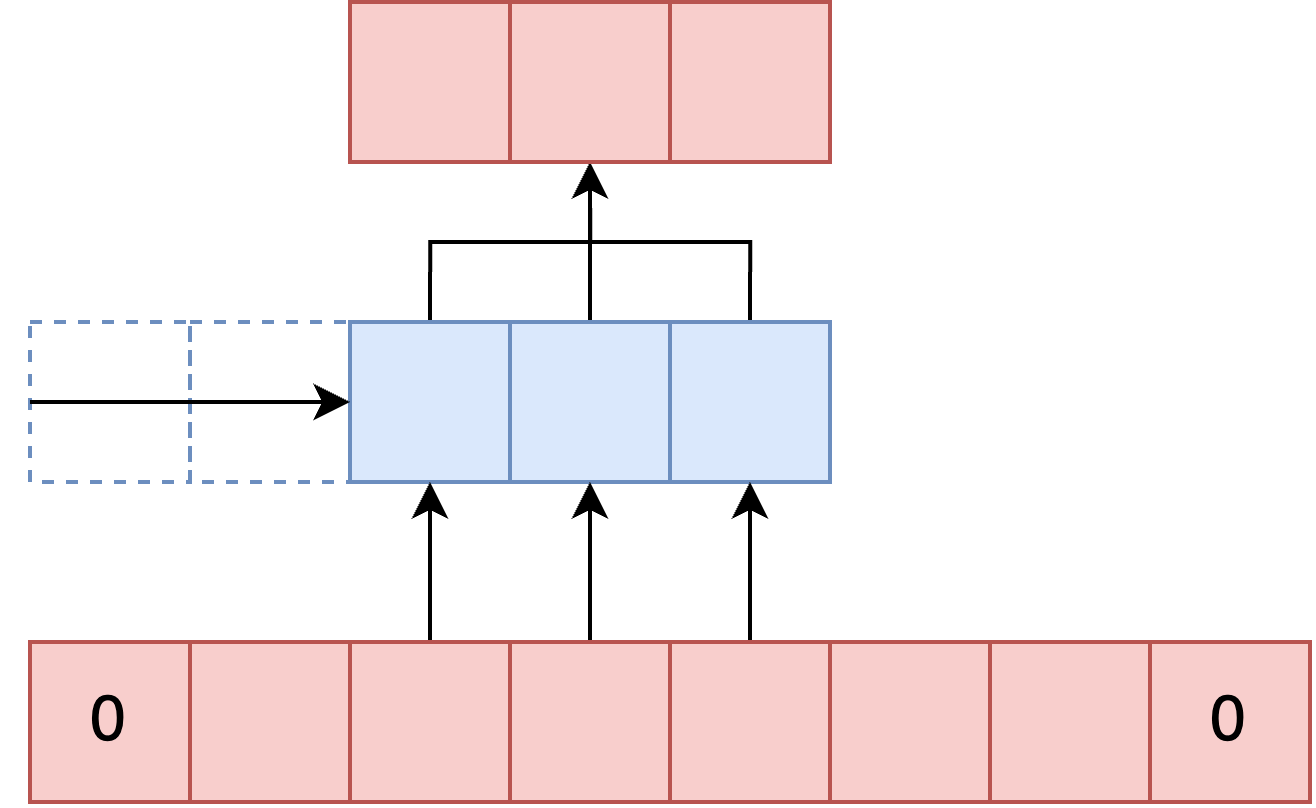
\includegraphics[height=4cm]{./figure/sec3/conv3.drawio.png}
        \caption{$\lr{\kernelSizeUpper, \strideUpper, \dilationUpper} = \lr{3, 2, 1}$}
        \label{sec3:fig:conv3}
    \end{subfigure}
    \begin{subfigure}[b]{0.48\textwidth}
        \centering
        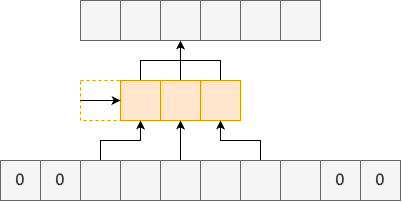
\includegraphics[height=4cm]{./figure/sec3/conv4.drawio.png}
        \caption{$\lr{\kernelSizeUpper, \strideUpper, \dilationUpper} = \lr{3, 1, 2}$}
        \label{sec3:fig:conv4}
    \end{subfigure}
    \caption{ある次元における一次元畳み込み層の処理.$\kernelSizeUpper$はカーネルサイズ,$\strideUpper$はストライド,$\dilationUpper$はダイレーションを表し,図中の0はパディング部を表す.}
    \label{sec3:fig:conv_variations}
\end{figure}

\subsubsection{転置畳み込み層}
転置畳み込み層は,畳み込み層の逆演算に対応する層であり,主に入力のアップサンプリングに使用される.図~\ref{sec3:fig:tconv_variations}に,ある入出力次元間における一次元転置畳み込み層の処理を示す.一次元転置畳み込み層では,$\timeLower$番目の入力とカーネルの積を計算し,その結果を$\timeLower$番目から$\timeLower + \kernelSizeUpper$番目までの出力とする.ここで$\kernelSizeUpper$はカーネルサイズである.また,複数の入力から計算された出力がオーバーラップする場合,これらは加算される.図~\ref{sec3:fig:tconv1}は,カーネルサイズを4,ストライドを1とした場合の様子である.アップサンプリングを行いたい場合は,ストライドを2以上とすれば良い.図~\ref{sec3:fig:tconv2}にカーネルサイズを4,ストライドを2とした場合を示す.この時,入力系列長が4であるのに対して,出力系列長が10まで拡大されていることがわかる.ここで,出力系列長を入力系列長の整数倍に保つためには,出力の両端の削除数を適切に設定する必要がある.上述の例では両端の削除数を1とすることで,出力系列長を入力系列長の2倍である8に調整できる.

\begin{figure}[tb]
    \centering
    \begin{subfigure}[b]{0.48\textwidth}
        \centering
        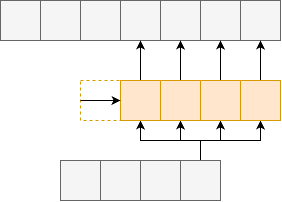
\includegraphics[height=4cm]{./figure/sec3/tconv1.drawio.png}
        \caption{$\lr{\kernelSizeUpper, \strideUpper} = \lr{4, 1}$}
        \label{sec3:fig:tconv1}
    \end{subfigure}
    \begin{subfigure}[b]{0.48\textwidth}
        \centering
        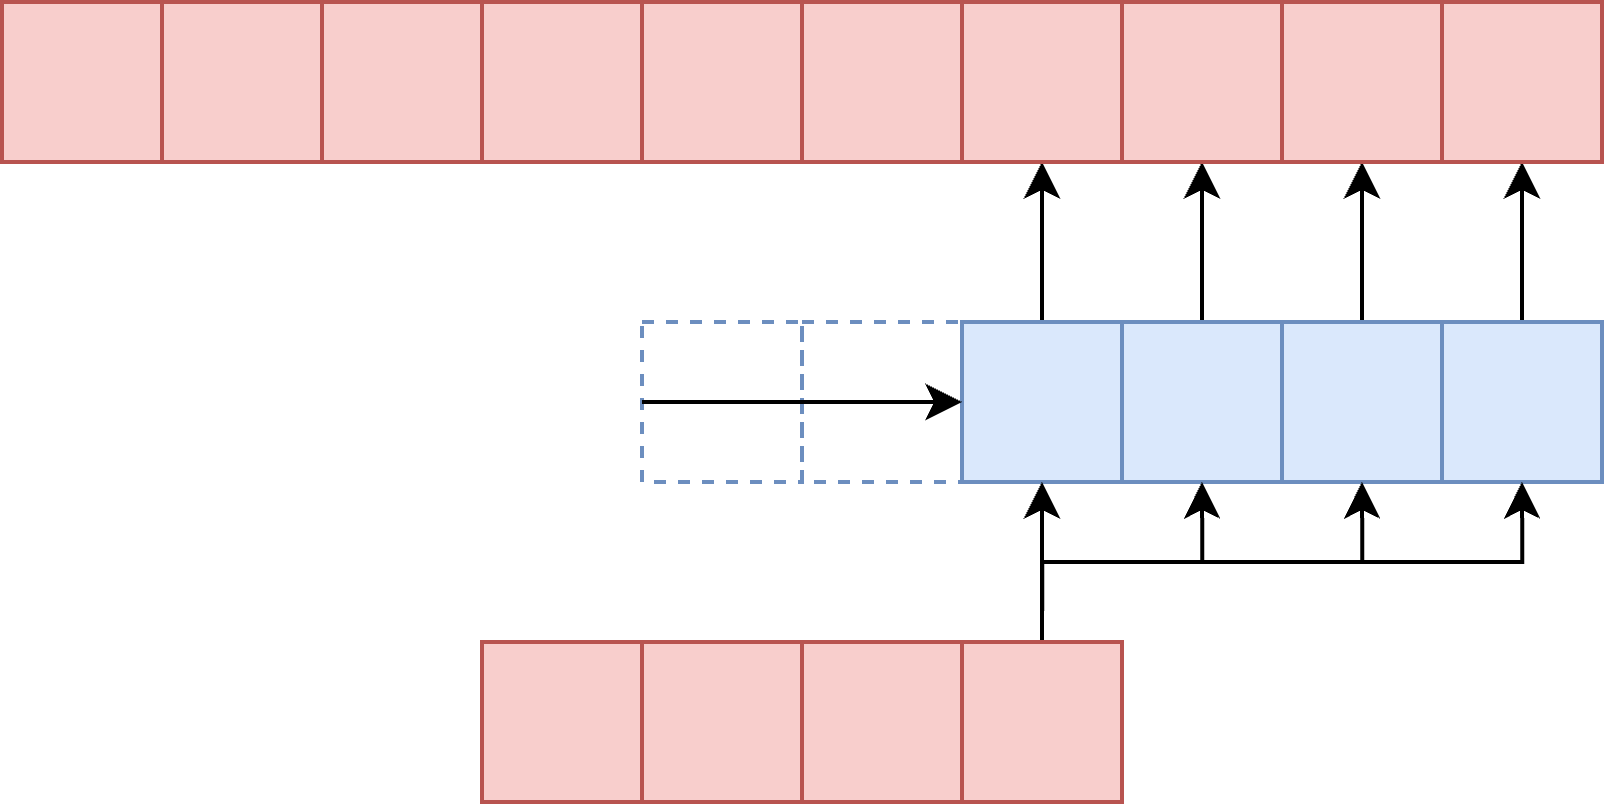
\includegraphics[height=4cm]{./figure/sec3/tconv2.drawio.png}
        \caption{$\lr{\kernelSizeUpper, \strideUpper} = \lr{4, 2}$}
        \label{sec3:fig:tconv2}
    \end{subfigure}
    \caption{ある次元における一次元転置畳み込み層の処理.$\kernelSizeUpper$はカーネルサイズ,$\strideUpper$はストライドを表す.}
    \label{sec3:fig:tconv_variations}
\end{figure}

\subsubsection{活性化関数}
活性化関数は,ニューラルネットワークの出力に非線形性を与えるための関数である.これにより,DNNは単純な線形変換だけでは表現できない複雑な入出力の関係を学習可能になる.以下,活性化関数への入力を$\inputLower \in \realSet$として,代表的なものを6つ述べる.また,本節で取り上げる活性化関数とその一階導関数のグラフを図~\ref{sec3:fig:activations_and_their_prime}に示す.

1つ目は,シグモイド関数である.シグモイド関数は
\begin{equation}
    \sigmoid\lr{\inputLower} = \frac{1}{1 + \exp\lr{-\inputLower}}
\end{equation}
で与えられ,その一階導関数は
\begin{equation}
    \dv{\sigmoid\lr{\inputLower}}{x} = \frac{\exp\lr{-\inputLower}}{\lr{1 + \exp\lr{-\inputLower}}^{2}}
\end{equation}
となる.図~\ref{sec3:fig:activations_prime}より,シグモイド関数の一階導関数の最大値は$\inputLower=0$における0.25であり,$\lrAbs{\inputLower - 0}$が大きくなるのに伴ってその値は小さくなることがわかる.DNNの各重みは,損失関数の勾配を利用することで更新されるから,シグモイド関数以前の層の重みにおける勾配は,シグモイド関数の一階導関数の値が乗算された結果となる.前述したように,シグモイド関数は一階導関数の値が小さくなりがちであるから,それ以前の層における勾配も小さくなり,重みの更新が進みづらくなる可能性がある.この問題を,勾配消失と呼ぶ.

2つ目は,$\tanh$関数である.$\tanh$は
\begin{equation}
    \tanh\lr{\inputLower} = \frac{\exp\lr{\inputLower} - \exp\lr{-\inputLower}}{\exp\lr{\inputLower} + \exp\lr{-\inputLower}}
\end{equation}
で与えられ,その一階導関数は
\begin{align}
    \dv{\tanh\lr{\inputLower}}{x} & = \frac{4}{\lr{\exp\lr{\inputLower} + \exp\lr{-\inputLower}}^{2}} \\
                                  & = \frac{1}{\cosh\lr{\inputLower}^{2}}
\end{align}
となる.$\tanh$の値域は$\lrClosedInterval{-1}{1}$となっており,図\ref{sec3:fig:activations_prime}より$\lrAbs{\inputLower - 0}$が小さいところではシグモイド関数より一階導関数の値が大きくなっていることがわかる.しかし,$\lrAbs{\inputLower - 0}$が大きくなればシグモイド関数と同様に一階導関数の値が小さく,勾配消失のリスクを抱えていることがわかる.

3つ目は,$\relu$である.$\relu$は
\begin{equation}
    \relu\lr{\inputLower} = \max \lr{0, \inputLower}
\end{equation}
で与えられ,その一階導関数は
\begin{equation}
    \dv{\relu\lr{\inputLower}}{x} =
    \begin{cases}
        1 & \text{if $\inputLower > 0$}  \\
        0 & \text{if $\inputLower <= 0$}
    \end{cases}
\end{equation}
となる.ここで,$\relu$は本来$x = 0$で微分不可能であるが,便宜上$\dv*{\relu\lr{0}}{x} = 0$とした.$\relu$は入力が0以上であれば恒等写像として振る舞うが,0未満であれば0に写す.一階導関数は0あるいは1のみを取り,特に入力が正の値であれば常に1となることから,シグモイド関数や$\tanh$よりも勾配消失が起こりづらい.$\relu$は現在,標準的な活性化関数として広く用いられている.しかし,$\relu$への入力が0未満の値を取るとき,$\relu$入力についての出力の勾配は0になるから,$\relu$以前の層の重みが更新されず,学習が遅くなる可能性がある.

3つ目は,$\leakyRelu$\cite{maas2013rectifier}である.$\leakyRelu$は
\begin{equation}
    \leakyRelu\lr{\inputLower} =
    \begin{cases}
        \inputLower  & \text{if $\inputLower > 0$}  \\
        a\inputLower & \text{if $\inputLower <= 0$}
    \end{cases}
\end{equation}
で与えられ,その一階導関数は
\begin{equation}
    \dv{\leakyRelu\lr{\inputLower}}{x} =
    \begin{cases}
        1 & \text{if $\inputLower > 0$}  \\
        a & \text{if $\inputLower <= 0$}
    \end{cases}
\end{equation}
となる.ここで,$\leakyRelu$は本来$x = 0$で微分不可能であるが,便宜上$\dv*{\leakyRelu\lr{0}}{x} = a$とした.ReLUと比較すると,0未満の入力に対しても0でない値を出力し,一階導関数も0にならない点が異なっている.これにより,重みの更新が進まなくなるReLUの課題を解消した.

5つ目は,$\prelu$\cite{he2015delving}である.これは,$\leakyRelu$と似た活性化関数であるが,$\leakyRelu$のパラメータ$a$を学習可能にすることで,その他の層と合わせて最適化が可能となったことが特徴である.

6つ目は,$\gelu$\cite{hendrycks2016gaussian}である.$\gelu$は
\begin{equation}
    \gelu\lr{\inputLower} = \inputLower \Phi\lr{\inputLower}
\end{equation}
で与えられる.ここで,
\begin{equation}
    \Phi\lr{\inputLower} = P\lr{X \le \inputLower}, ~ X \sim \mathcal{N} \lr{0, 1}
\end{equation}
である.$\gelu$の一階導関数は,
\begin{equation}
    \dv{\gelu\lr{\inputLower}}{x} = \Phi\lr{\inputLower} + \frac{\inputLower}{\sqrt{2\pi}}\exp\lr{-\frac{\inputLower^{2}}{2}}
\end{equation}
となる.$\gelu$は,$\relu$が入力に対して0あるいは1を確定的にかける活性化関数と捉えた上で,これを入力に依存した確率的な挙動に変更したものである.
% 実際,$\binaryMaskLower \sim \text{Bernoulli}\lr{\Phi\lr{\inputLower}}$とすると,
% \begin{align}
%     \gelu\lr{\inputLower} & = \inputLower \Phi\lr{\inputLower}                                                             \\
%                           & = 1 \inputLower \cdot \Phi\lr{\inputLower} + 0 \inputLower \cdot \lr{1 - \Phi\lr{\inputLower}} \\
%                           & = \expectation{mx}
% \end{align}
% となり,$\gelu$の出力は確率的なバイナリマスク$\binaryMaskLower$を入力$\inputLower$にかけた,$mx$の期待値に等しいことがわかる.

\begin{figure}[tb]
    \centering
    \begin{subfigure}[b]{1.0\textwidth}
        \centering
        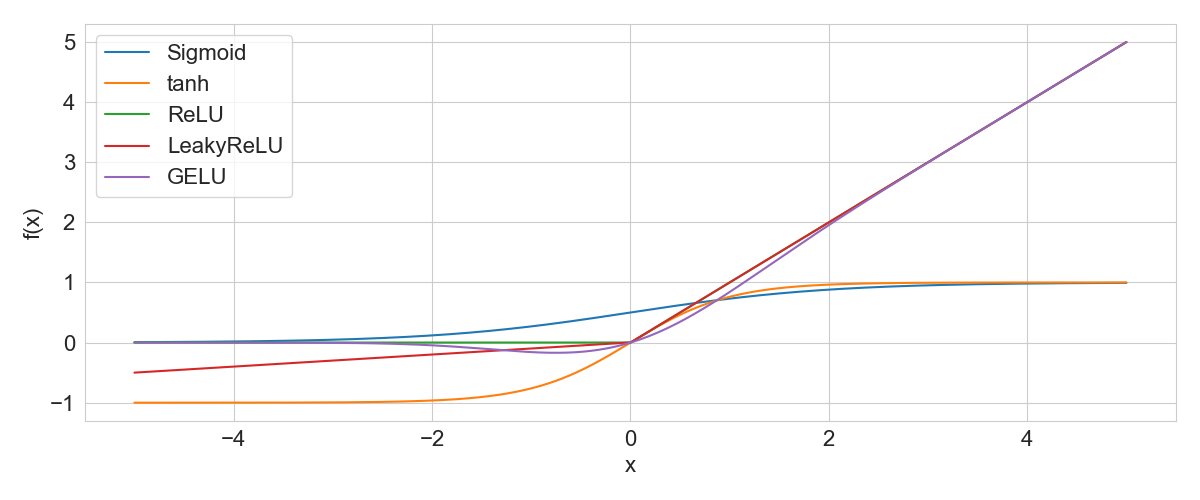
\includegraphics[height=6cm]{./figure/sec3/activations.png}
        \caption{活性化関数}
        \label{sec3:fig:activations}
    \end{subfigure}
    \begin{subfigure}[b]{1.0\textwidth}
        \centering
        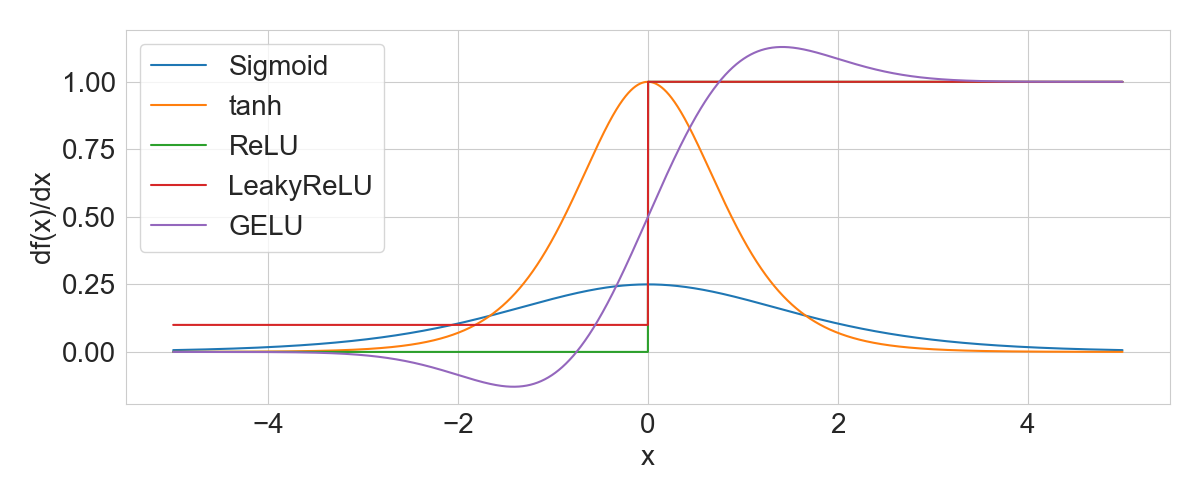
\includegraphics[height=6cm]{./figure/sec3/activations_prime.png}
        \caption{活性化関数の一階導関数}
        \label{sec3:fig:activations_prime}
    \end{subfigure}
    \caption{活性化関数の例}
    \label{sec3:fig:activations_and_their_prime}
\end{figure}

\subsubsection{再帰型ニューラルネットワーク}
再帰型ニューラルネットワーク(Recurrent Neural Network; RNN)は,自身の過去の出力を保持し,それをループさせる再帰的な構造を持ったネットワークである.

近年よく用いられるRNNとして,長・短期記憶(Long Short-Time Memory; LSTM)\cite{hochreiter1997long}がある.LSTMは入力ゲート,忘却ゲート,出力ゲートの3つを持ち,これらゲートによってネットワーク内部の情報の取捨選択を行うことで,長い系列データからの学習を可能にした.LSTMのネットワーク内部で行われる計算を以下に示す.
\begin{gather}
    \bm{f}_{\timeLower} = \sigmoid\lr{\fcLayerValue{\bm{\inputLower}_{\timeLower}}{\bm{\weightAndBias}_{f, x}} + \fcLayerValue{\bm{h}_{\timeLower-1}}{\bm{\weightAndBias}_{f, h}}} \\
    \bm{i}_{\timeLower} = \sigmoid\lr{\fcLayerValue{\bm{\inputLower}_{\timeLower}}{\bm{\weightAndBias}_{i, \inputLower}} + \fcLayerValue{\bm{h}_{\timeLower-1}}{\bm{\weightAndBias}_{i, h}}} \\
    \tilde{\bm{c}}_{\timeLower} = \tanh\lr{\fcLayerValue{\bm{\inputLower}_{\timeLower}}{\bm{\weightAndBias}_{\tilde{c}, \inputLower}} + \fcLayerValue{\bm{h}_{\timeLower-1}}{\bm{\weightAndBias}_{\tilde{c}, h}}} \\
    \bm{o}_{\timeLower} = \sigmoid\lr{\fcLayerValue{\bm{\inputLower}_{\timeLower}}{\bm{\weightAndBias}_{o, \inputLower}} + \fcLayerValue{\bm{h}_{\timeLower-1}}{\bm{\weightAndBias}_{o, h}}} \\
    \bm{c}_{\timeLower} = \bm{f}_{\timeLower} \elemMul \bm{c}_{\timeLower-1} + \bm{i}_{\timeLower} \elemMul \tilde{\bm{c}}_{\timeLower} \\
    \bm{h}_{\timeLower} = \bm{o}_{\timeLower} \elemMul \tanh\lr{\bm{c}_{\timeLower}}
\end{gather}
ここで,$\bm{\inputLower}_{\timeLower} \in \realSet^{\dimUpper_{\text{in}}}$は時刻$\timeLower$の入力,$\bm{f}_{\timeLower} \in \lrsq{0, 1}^{\dimUpper_{\text{out}}}$は忘却ゲートの出力,$\bm{i}_{\timeLower} \in \lrsq{0, 1}^{\dimUpper_{\text{out}}}$は入力ゲートの出力,$\bm{c}_{\timeLower} \in \lrsq{-1, 1}^{\dimUpper_{\text{out}}}$は時刻$\timeLower$におけるセルの状態,$\bm{o}_{\timeLower} \in \lrsq{0, 1}^{\dimUpper_{\text{out}}}$は出力ゲートの出力,$\bm{h}_{\timeLower} \in \lrsq{-1, 1}^{\dimUpper_{\text{out}}}$は時刻$\timeLower$における隠れ状態,$\dimUpper_{\text{in}}, \dimUpper_{\text{out}}$は特徴量の次元を表す.また,$\concat{\cdot, \ldots, \cdot}$は入力された特徴量の次元方向の結合,$\elemMul$は要素積を表す.忘却ゲート出力$\bm{f}_{\timeLower}$が前時刻のセル状態$\bm{c}_{\timeLower - 1}$に含まれる情報の選択,入力ゲート出力$\bm{i}_{\timeLower}$が新たな入力$\tilde{\bm{c}}_{\timeLower}$に含まれる情報の選択に用いられ,$\bm{c}_{\timeLower}$が決まる.その後,出力ゲート出力$\bm{o}_{\timeLower}$が$\bm{c}_{\timeLower}$に含まれる情報の選択に用いられ,$\bm{h}_{\timeLower}$が決まる.

また,LSTMが3つのゲートを必要とするのに対し,ゲートを2つに減らすことでネットワークの軽量化を図ったのがゲート付き回帰型ユニット(Gated Recurrent Unit; GRU)\cite{cho2014learning}である.GRUはリセットゲートと更新ゲートの2つを用いて隠れ状態を更新する.GRUのネットワーク内部で行われる計算を以下に示す.
\begin{gather}
    \bm{z}_{\timeLower} = \sigmoid\lr{\fcLayerValue{\bm{\inputLower}_{\timeLower}}{\bm{\weightAndBias}_{z, \inputLower}} + \fcLayerValue{\bm{h}_{\timeLower-1}}{\bm{\weightAndBias}_{z, h}}} \\
    \bm{r}_{\timeLower} = \sigmoid\lr{\fcLayerValue{\bm{\inputLower}_{\timeLower}}{\bm{\weightAndBias}_{r, \inputLower}} + \fcLayerValue{\bm{h}_{\timeLower-1}}{\bm{\weightAndBias}_{r, h}}} \\
    \tilde{\bm{h}}_{\timeLower} = \tanh\lr{\fcLayerValue{\bm{\inputLower}_{\timeLower}}{\bm{\weightAndBias}_{\tilde{h}, \inputLower}} + \bm{r}_{\timeLower} \elemMul \fcLayerValue{\bm{h}_{\timeLower-1}}{\bm{\weightAndBias}_{\tilde{h}, h}}} \\
    \bm{h}_{\timeLower} = \lr{1 - \bm{z}_{\timeLower}} \elemMul \bm{h}_{\timeLower-1} + \bm{z}_{\timeLower} \elemMul \tilde{\bm{h}}_{\timeLower}
\end{gather}
ここで,$\bm{x}_{\timeLower} \in \realSet^{\dimUpper_{\text{in}}}$が時刻$\timeLower$における入力,$\bm{z}_{\timeLower} \in \lrsq{0, 1}^{\dimUpper_{\text{out}}}$が更新ゲートの出力,$\bm{r}_{\timeLower} \in \lrsq{0, 1}^{\dimUpper_{\text{out}}}$がリセットゲートの出力,$\bm{h}_{\timeLower} \in \lrsq{-1, 1}^{\dimUpper_{\text{out}}}$が時刻$\timeLower$における隠れ状態を表す.更新ゲート出力$\bm{z}_{\timeLower}$が$\bm{h}_{\timeLower - 1}$と$\tilde{\bm{h}}_{\timeLower}$に含まれる情報の選択,リセットゲート出力$\bm{r}_{\timeLower}$が$\bm{h}_{\timeLower - 1}$に含まれる情報の選択に用いられる.

\subsubsection{正規化層}
DNNの学習過程では学習の進行に伴って重みが変化するため,その度に各層への入力の分布が変わってしまう.これは内部共変量シフトと呼ばれ,ネットワークの学習を不安定にする原因となる.これに対し,バッチ正規化(Batch Normalization)\cite{ioffe2015batch}が有効である.バッチ正規化は,ミニバッチ内における入力特徴量の期待値と分散を次元ごとに計算し,これらを用いて入力特徴量を次元ごとに標準化するものである.ここで,バッチサイズを$\numUpper$,バッチ正規化への$D$次元の入力特徴量を$\bm{\inputLower}_{\numLower} \in \realSet^{\dimUpper} ~ \lr{\numLower = 1, \ldots, \numUpper}$,出力特徴量を$\bm{y}_{\numLower} \in \realSet^{\dimUpper} ~ \lr{\numLower = 1, \ldots, \numUpper}$とする.このとき,各$\numLower$に対し入力特徴量$\bm{\inputLower}_{\numLower}$の$\dimLower$次元目の成分を$\inputLower_{\numLower, \dimLower}$,出力特徴量$\bm{\outputLower}_{\numLower}$の$\dimLower$次元目の成分を$\outputLower_{\numLower, \dimLower}$とすると,$\outputLower_{\numLower, \dimLower}$は
\begin{align}
    \mean^{B}_{\dimLower}                      & = \frac{1}{\numUpper} \sum_{\numLower = 1}^{\numUpper} \inputLower_{\numLower, \dimLower}                                  \\
    \lr{\std^{B}_{\dimLower}}^{2}              & = \frac{1}{\numUpper} \sum_{\numLower = 1}^{\numUpper} \lr{\inputLower_{\numLower, \dimLower} - \mean^{B}_{\dimLower}}^{2} \\
    \tilde{\inputLower}_{\numLower, \dimLower} & = \frac{\inputLower_{\numLower, \dimLower} - \mean^{B}_{\dimLower}}{\sqrt{\lr{\std^{B}_{\dimLower}}^{2} + \epsilon}}       \\
    \outputLower_{\numLower, \dimLower}        & = \normScale_{\dimLower} \tilde{\inputLower}_{\numLower, \dimLower} +  \normShift_{\dimLower}
\end{align}
で与えられる.ここで,$\normScale_{\dimLower}, \normShift_{\dimLower}$は学習可能なスカラーであり,$\epsilon$はゼロ割を避けるためのスカラーである.バッチ正規化では$\normScale_{\dimLower}, \normShift_{\dimLower}$によって表現力を向上させており,実際
\begin{align}
    \normScale_{\dimLower} & = \sqrt{\lr{\std^{B}_{\dimLower}}^{2} + \epsilon} \\
    \beta_{\dimLower}      & = \mean^{B}_{\dimLower}
\end{align}
とすれば,標準化前の入力を再び得ることが可能である.学習時は,サンプルの標準化に用いる統計量とは別に,期待値の移動平均と不偏分散の移動平均を計算しておく.推論時は学習終了時に得られたこれら移動平均の値を用いるため,入力サンプルによらない挙動になる.

バッチ正規化はDNNの学習の安定化に貢献する一方,ミニバッチ全体における統計量を利用するため,バッチサイズが小さい場合はデータの分布を安定させることが難しくなる.また,テキストや音声といった系列長を持つデータを扱う場合,ミニバッチを構成するためにはゼロパディングによって系列長を揃える必要がある.この時,RNNの各ステップの出力に対しバッチ正規化を適用すると,ゼロパディングによって人為的に系列量を揃えているから,統計量が実際のデータの分布からかけ離れたものになる可能性がある.これら課題に対し,ミニバッチ内の各サンプルごとに期待値と分散を求めて標準化する,レイヤー正規化(Layer Normalization)\cite{ba2016layer}がある.バッチ正規化のときと同様の表記を用いると,$\outputLower_{\numLower, \dimLower}$は
\begin{align}
    \mean^{L}_{\numLower}                      & = \frac{1}{\dimUpper} \sum_{\dimLower = 1}^{\dimUpper} \inputLower_{\numLower, \dimLower}                                  \\
    \lr{\std^{L}_{\numLower}}^{2}              & = \frac{1}{\dimUpper} \sum_{\dimLower = 1}^{\dimUpper} \lr{\inputLower_{\numLower, \dimLower} - \mean^{L}_{\numLower}}^{2} \\
    \tilde{\inputLower}_{\numLower, \dimLower} & = \frac{\inputLower_{\numLower, \dimLower} - \mean^{L}_{\numLower}}{\sqrt{\lr{\std^{L}_{\numLower}}^{2} + \epsilon}}       \\
    \outputLower_{\numLower, \dimLower}        & = \normScale_{\dimLower} \tilde{\inputLower}_{\numLower, \dimLower} +  \normShift_{\dimLower}
\end{align}
で与えられる.

上述したバッチ正規化およびレイヤー正規化は,特徴量を標準化することで学習を安定させる手法であった.一方,DNN内のある層の重みを再パラメータ化することで学習を安定させる手法として,重み正規化(Weight Normalization)\cite{salimans2016weight}がある.これは,ある層の重みベクトル$\bm{\weightLower}$を,
\begin{equation}
    \bm{\weightLower} = \frac{\bm{v}}{\lrTwoNorm{\bm{v}}} g
\end{equation}
のように単位ベクトル$\bm{v} / \lrTwoNorm{\bm{v}}$(ベクトルの向き)とスカラー$g$(ベクトルの長さ)に再パラメータ化するものである.学習時は重みの更新を$\bm{v}$と$g$で別々に行う.重み正規化は,バッチ正規化やレイヤー正規化と同様に学習の安定化に役立つが,計算に入力特徴量の系列長が依存しない.そのため,例えば音声波形など系列長が非常に長くなりがちなデータを扱う場合,計算コストを下げながら同様の効果を狙える手段だと考えられる.

\subsubsection{Transformer}
Transformer\cite{vaswani2017attention}は,自己注意機構(Self-Attention)を用いて,入力系列全体に渡る依存関係を捉えることができるニューラルネットワークである.特に,再帰的な計算を必要とするRNNと比較して,Transformerは並列計算のみ行うため,GPUによる計算の高速化が可能である.以下,入力特徴量を$\bm{\inputUpper} \in \realSet^{\timeUpper \times \dimUpper_{\text{model}}}$として,Transformerにおいて行われる計算を説明する.$T$は系列長,$\dimUpper_{\text{model}}$は特徴量の次元を表す.また,Transformer層の構造を図~\ref{sec3:fig:transformer_layer}に示す.

\begin{figure}[bt]
    \centering
    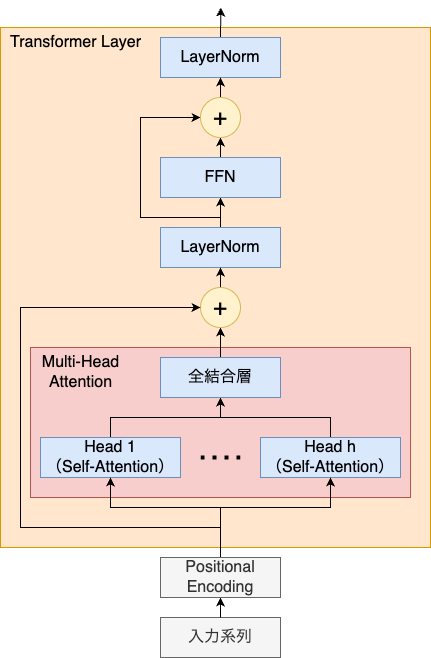
\includegraphics[height=140mm]{./figure/sec3/transformer.drawio.png}
    \caption{Transformer層の構造}
    \label{sec3:fig:transformer_layer}
\end{figure}

まず,TransformerにおけるSelf-Attentionの計算の流れを述べる.ここでは,はじめにクエリ$\bm{Q} \in \realSet^{\timeUpper \times \dimUpper_{k}}$,キー$\bm{K} \in \realSet^{\timeUpper \times \dimUpper_{k}}$,バリュー$\bm{V} \in \realSet^{\timeUpper \times \dimUpper_{v}}$の計算を行う.これは,
\begin{align}
    \bm{Q} & = \fcLayerValue{\bm{\inputUpper}}{\bm{\weightAndBias}_{Q}} \\
    \bm{K} & = \fcLayerValue{\bm{\inputUpper}}{\bm{\weightAndBias}_{K}} \\
    \bm{V} & = \fcLayerValue{\bm{\inputUpper}}{\bm{\weightAndBias}_{V}}
\end{align}
で与えられる.次に,クエリとキーを元にアテンション重みを求め,バリューに対する行列積を計算する.これは,
\begin{equation}
    \text{SA}\lr{\bm{Q}, \bm{K}, \bm{V}} = \text{softmax}\lr{\frac{\bm{Q}\bm{K}^\top}{\sqrt{\dimUpper_{k}}}} \bm{V}
\end{equation}
で与えられる.softmax関数は行方向に適用されるため,$\text{softmax}\lr{\bm{Q}\bm{K}^\top / \sqrt{\dimUpper_{k}}}$の各行ベクトルが,各クエリ$\bm{q}_{t} \in \realSet^{\dimUpper_{k}}$からキー$\bm{k}_{t} \in \realSet^{\dimUpper_{k}} ~ \lr{t = 1, \ldots, T}$に対する注意度になっている.

ここまでがSelf-Attentionの計算であったが,TransformerではSelf-Attentionを複数のヘッドで並列に計算し,各ヘッドの出力を結合して最終出力を得るMulti-Head Attentionが採用されている.これは,ヘッド数を$\numHeadUpper$とし,各ヘッド$\numHeadLower$におけるクエリ$\bm{Q}^{\numHeadLower} \in \realSet^{\timeUpper \times \frac{\dimUpper_{k}}{\numHeadUpper}}$,キー$\bm{K}^{\numHeadLower} \in \realSet^{\timeUpper \times \frac{\dimUpper_{k}}{\numHeadUpper}}$,バリュー$\bm{V}^{\numHeadLower} \in \realSet^{\timeUpper \times \frac{\dimUpper_{v}}{\numHeadUpper}}$によって計算された$\text{SA}\lr{\bm{Q}^{\numHeadLower}, \bm{K}^{\numHeadLower}, \bm{V}^{\numHeadLower}}$を用いて,
\begin{equation}
    \text{MHA}\lr{\bm{Q}, \bm{K}, \bm{V}} = \fcLayerValue{\concat{\text{SA}\lr{\bm{Q}^{\numHeadLower}, \bm{K}^{\numHeadLower}, \bm{V}^{\numHeadLower}}, \ldots, \text{SA}\lr{\bm{Q}^{\numHeadLower}, \bm{K}^{\numHeadLower}, \bm{V}^{\numHeadLower}}}}{\bm{\weightAndBias}_{\text{MHA}}}
\end{equation}
で与えられる.Multi-Head Attention後は,残差結合とレイヤー正規化を適用する.すなわち,この出力$\bm{\outputUpper} \in \realSet^{\timeUpper \times \dimUpper_{\text{model}}}$は,
\begin{equation}
    \bm{\outputUpper} = \text{LayerNorm}\lr{\text{MHA}\lr{\bm{Q}, \bm{K}, \bm{V}} + \bm{\inputUpper}}
\end{equation}
で与えられる.その後,全結合層を通し,再度残差結合とレイヤー正規化を適用することでTransformer層最終出力を得る.すなわち,
\begin{equation}
    \bm{\outputUpper} = \text{LayerNorm}\lr{\fcLayerValue{\relu\lr{\fcLayerValue{\bm{\outputUpper}}{\bm{\weightAndBias}_{1}}}}{\bm{\weightAndBias}_{2}} + \bm{\outputUpper}}
\end{equation}
となる.Transformer全体は,Transformer層を多層積み重ねて構成される.

最後に,TransformerではRNNと違い,並列計算によって系列全体を一度に処理することが可能であるが,それと引き換えに入力の順序情報を考慮することができなくなる.これに対し,TransformerではPositional Encodingによって入力に位置情報を与える.Positional Encodingは$\sin$と$\cos$に基づいて,
\begin{equation}
    \text{PositionalEncoding}\lr{\timeLower, \dimLower} =
    \begin{cases}
        \sin \lr{\frac{\timeLower}{10000^{2\dimLower / \dimUpper_{\text{model}}}}} & \text{if $d \bmod 2 = 0$} \\
        \cos \lr{\frac{\timeLower}{10000^{2\dimLower / \dimUpper_{\text{model}}}}} & \text{if $d \bmod 2 = 1$}
    \end{cases}
\end{equation}
で与えられる.
